\subsection{Wah-Wah}

The effect takes the original signal and mix it with another signal that passes through a bandpass filter. The bandpass filter is time varying, which means that it changes its position in the frequency spectrum. \\
Different parameters can be changed on the \gls{lfo} to customize the effect:\\

\begin{itemize}
	\item \textbf{The \gls{lfo} frequency}: it sets the speed at which the bandpass filter moves in the frequency spectrum.
	\item \textbf{\gls{lfo} start phase}: Determine where should the bandpass filter start.
	\item \textbf{\gls{lfo} depth}: the range of frequencies it should work on, high depth gives a bigger range and vice versa.
\end{itemize}

A block diagram of the effect is illustrated in \autoref{fig:wah_diag}.  

\begin{figure} [htbp]
	\centering
\begin{picture}(0,0)%
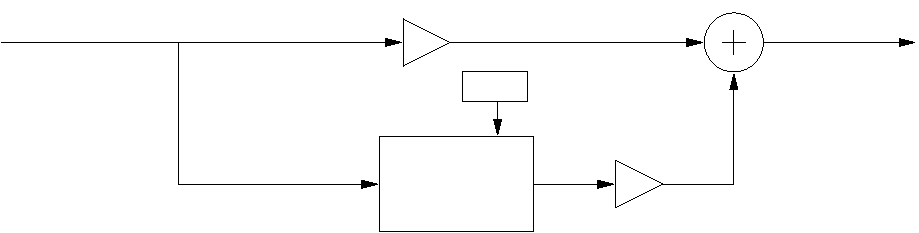
\includegraphics{wah_diag.pdf}%
\end{picture}%
\setlength{\unitlength}{4144sp}%
%
\begingroup\makeatletter\ifx\SetFigFont\undefined%
\gdef\SetFigFont#1#2#3#4#5{%
  \reset@font\fontsize{#1}{#2pt}%
  \fontfamily{#3}\fontseries{#4}\fontshape{#5}%
  \selectfont}%
\fi\endgroup%
\begin{picture}(6999,1977)(2689,-2233)
\put(5626,-1816){$Bandpass-$}%
\put(2791,-601){$Input$}%
\put(7021,-1501){\textit{Wah-Wah Mixer}}%
\put(5100,-421){\textit{Original Signal Mixer}}%
\put(8941,-601){$Output$}%
\put(5626,-2041){$Filter$}%
\end{picture}%


	\caption{Block diagram of the wah-wah effect}
	\label{fig:wah_diag}
\end{figure}

The phaser effect can be created by using a band-stop filter instead of a bandpass filter using the same block diagram presented in \autoref{fig:wah_diag}.

There is another type of wah-wah effect called M-fold wah-wah which uses multiple M-tap bandpass filters that move around the spectrum at the same time.

An example of a time domain response is shown in figure \autoref{fig:wah-wah-response}.

\begin{figure} [htbp!]
	\centering
	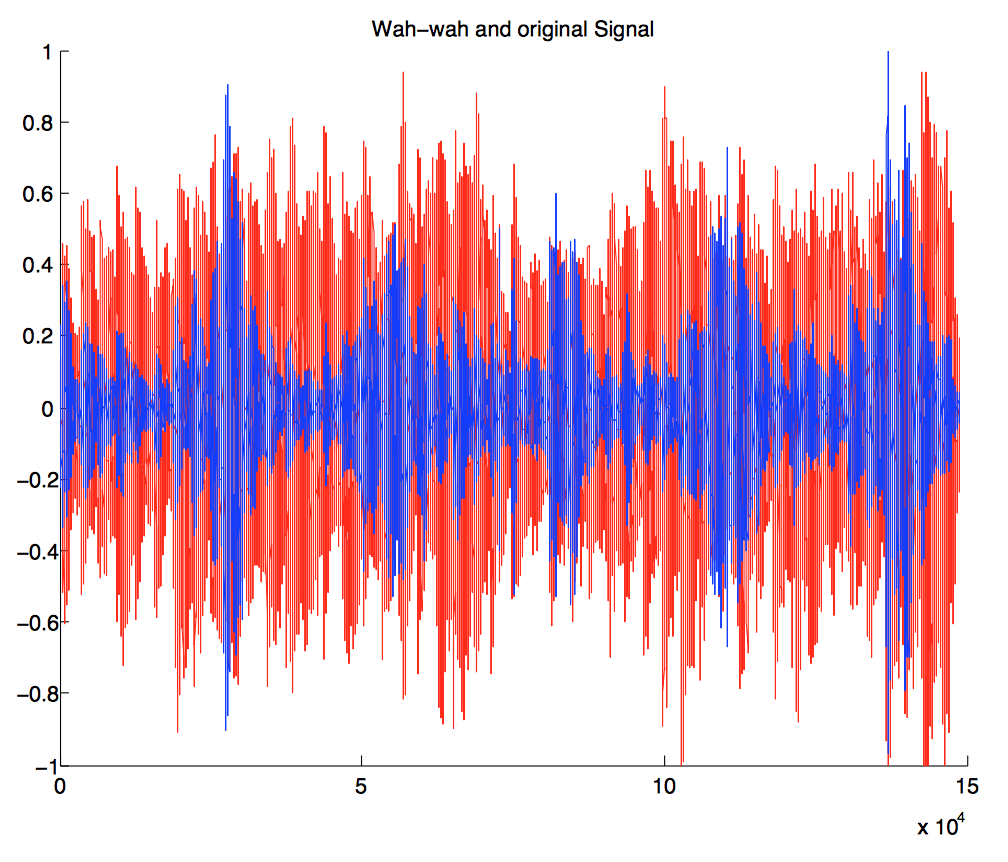
\includegraphics[width=0.6\textwidth]{wah-wah-response.png}
	\caption{Time domain response of the original sound (red) and the one after having the wah-wah effect (blue)}
	\label{fig:wah-wah-response}
\end{figure}

\todo[inline]{Jonas: Muhammed, can you explain the above time domain spectra?(and the block diagram)}
